\documentclass[10pt]{article}

\usepackage{geometry,amsthm,amsmath,amssymb,tikz,fancyhdr,float}

\def\real{\mathbb{R}}
\def\q{\mathbb{H}}
\def\bv{\text{\textbf{v}}}
\def\bi{\text{\textbf{i}}}
\def\bj{\text{\textbf{j}}}
\def\bk{\text{\textbf{k}}}


\title{\textbf{The Asteria 3D Game Engine} \\ \textbf{\small Architecture Document } }
\author{Samuel C. Payson \and Akanksha Vyas}

\begin{document}
\maketitle

\begin{center}
   \begin{tikzpicture}
      
   \end{tikzpicture}
\end{center}

\thispagestyle{empty}
\pagebreak
\pagenumbering{roman}
\setcounter{page}{1}
\tableofcontents

\pagebreak
\pagenumbering{arabic}
\setcounter{page}{1}

\part*{An Introduction To Asteria}

\section{What is Asteria?}
Asteria is a 3D game engine being developed by members of the Clarkson Open
Source Institute at Clarkson University in Potsdam, NY. The project aims to be
a high-performance, open-source game engine with a clean and comprehensible
design.

The goals of this project are to build a high performance open source game
engine where components are designed to be orthogonal.

This documents describes major design decisions and the motivations behind them.
It then describes the overall structure of the project, followed by
implementation level descriptions of its subsystems.

\section{Licencing Information}

\pagebreak

\part*{High-Level Design}

\section{Software Design}

\section{The Subsystems}

The current implementation of Asteria has an animation subsystem and a resource
management subsystem.  


\part*{The Subsystems}
\section{The Animation Subsystem}
The animation subsystem parses a text-based description of a animated 3D model
and draws it to the screen. It is currently implemented for the md5 file format
popularized by Doom-3 (completely unrelated to the md5 cryptographic hash).
Consistent with the md5 file format, it performs skeletal animation using vertex 
skimming. The animation subsystem has three components: the parser, the draw 
function and the shaders.

The parser is responsible for parsing a md5 file and storing its description.
The draw function is responsible for calculating the exact coordinates of each
joint in the frame. The shaders use vertex skimmimg to actually draw the object. 

\subsubsection*{md5 File Format}
Animation of objects in md5 files is represented by the position and orientation
of every joint of the object at regular intervals. Different frame characterrize
thses different intervals. The file contains a base frame, 
describing one such the orientation and position for each joint. All successive 
frames represent the joints as offsets from the base frame. The file also contains 
a hirarchy of dependencies for each joint, the frame rate of the animation, and 
the total number of frames, joints and animated components. More information on
the file format can be found at
\textit{http://tfc.duke.free.fr/coding/md5-specs-en.html}.

For the current implementation, we are assuming that all objects are created in
Blender. Blender is free and open source software for creating 3D objects. It is
a common substitute for industry standerd Maya. More information on Blender can
be found at \textit{www.blender.org/}.

\subsection{The Parser}
As the name suggests, this component parses the animation file. It uses Flex and
Bison, tools for generating scanners and parsers efficiently. More information
on these can be found at \\\textit{http://dinosaur.compilertools.net/}. From the offsets
and the base frame values, the parser calculates the position and orientation for each
joint in every frame. From the hierarchy description, it calculates the parent of each joint.

md5 files use vectors in $\mathbb{R}^3$ to represent position and quaternions to
represent orientation. Quaternions are an algebraic structure that are found to
be very nifty for computer graphics. A description of the structure can be found
in the appendix, but for simplicity we can just look at them as vectors in
$\mathbb{R}^4$.

The animation subsystem populates the md5AnimData struct that can be
found in \\ \textit{/include/md5Structures.h}. Each joint has a position vector, an
orientation quaternion and a parent. If it is a root joint the parent is set to
-1.

\subsection{The Draw Function}
The draw function has two parts. The first part, given a time uses the framerate
to calculate which two frames the animation is currently between, and how far
between them it is. With this information it interpolates between the two frames to
calculate the position and orientation of each joint at that instant. A more
detailed description of interpolation techniques will follow. 

Every joint will be affected by any change in the orientation of its parent. 
The draw function need to change the position and orientation of a joint with 
respect to the orientation of its parent. The second part takes care of this. 
Assuming a topologically sorted list of joints (as Blender guarantees), it starts
from the top and rotates the position and orientation of every joint by the
orientation of its parent. Now it is ready draw these points. It sends the
position of each joint to the shaders, which then take care of this.

\subsubsection{Interpolation Techniques}
Interpolation techniques help identify a smooth path between the two frames. 
Given two vectors or quaternions they attempt to find a third vector or quaternion on this
path respectively. The draw function uses linear interpolation (LERP) for the
position vectors and a modified version of normalized linear interpolation
(NLERP) for rotation quaternions. More information on these can be found in the
appendix.

\subsection{Shaders}

\appendix
\section{The Quaternion Algebraic Structure}
Quaternions were invented by Irish mathematician Sir William Rowan Hamilton in
1843. They have been found to be useful in many fields of mathematics and computer
science, including 3D graphics.
Quaternions form a number system that extends the complex numbers into four
dimensions. A quaternion is of the form: \[ a + b\bi + c\bj + d\bk, \] \[ \text{where
} a,b,c,d \in \real \text{ and } \bi^2 = \bj^2 = \bk^2 = \bi\bj\bk = -1 \] \[ \text{ also, }
\bi\bj = \bk = -\bj\bi, \bj\bk = \bi = -\bk\bj, \bk\bi = \bj = -\bi\bk \]
They common notation for q is $[s,\bv]$, where $s \in \real $, $\textbf{v} \in
\real^3$ and $\bi, \bj, \bk$ are imaginary numbers. 

\section{More About Interpolation}
   
Now lets talk about interpolation techniques. Three 
common interpolation techniques are discussed. 
\begin{enumerate}
\item Linear Interpolation (LERP) is the simplest interpolation technique. The
idea is to draw a line between two points and find a third point at the desired
distance between them. Though this is useful for interpolating between position
vectors, it is graphically inaccurate for quaternions. Let $v_1, v_2, t$ where $v_1, v_2$ 
are the vectors describing the position you want to interpolate between, and $t$ 
is the distance between them. Equation~\ref{e1} describes the math. 

\begin{align}
\label{e1}
(1-t)q_1 + tq_2
\end{align}

\item 
Spherical linear interpolation (SLERP) was the next technique we looked at. It
is currently the most popular interpolation technique. SLERP calculates the
point on the arc of a circle at the desired distance between two quaternions.
Figure~\ref{f1} gives us an idea of what this looks like.

\begin{figure}[H]
   \begin{center}
      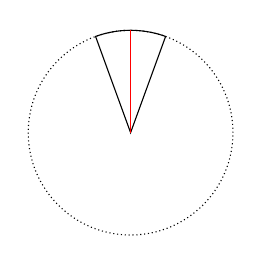
\begin{tikzpicture}
         \draw (0,0) -- (110:1.3cm) arc (110:70:1.3cm) -- cycle;
         \draw (0,0) -- (90:1.3cm) [red];
         \draw (0,0) circle (1.3cm) [densely dotted];
      \end{tikzpicture}
      \caption{Quaternions rotating around a pivot}
      \label{f1}
   \end{center}
\end{figure}

Let $q_1, q_2, t$, where $q_1, q_2$ are the quaternions you want to interpolate
between and $t$ is the distance between them. Equation~\ref{e2} describes the math. 

\begin{align}
\label{e2}
q_1(q_1*q_2)^t
\end{align}

A more implementation-friendly version of the math can be found at
\textit{vMath.c}.

The problem with SLERP is that its computationally expensive. 

\item
Normalized linear interpolation (NLERP) is a fairly new interpolations
technique that tries to balance the positives and negatives LERP and
SLERP. The basic idea is to do the LERP operation and then normalize the result.

Let $q_1, q_2, t$, where $q_1, q_2$ are the quaternions you want to interpolate
between and $t$ is the distance between them. Equation~\ref{e3} describes the math. 

\begin{align}
\label{e3}
norm((1-t)q_1 + tq_2)
\end{align}

Intuitively this seems like it would be much faster and graphically correct.
However, we encountered a problem with it. We realized that you need ensure
that the cosine of the angles between the two quaternions is positive.
On encountering a negative value, you have to negate one of the quaternions in
order for it to interpolate along the correct arc. This increases
that computation significantly, making it only marginally faster than SLEPR, if
at all. We are currently looking for a more efficient way to do this check.
\end{enumerate}

\end{document}
